\documentclass{article}
\usepackage[utf8]{inputenc}
\usepackage[spanish]{babel}
\usepackage{listings}
\usepackage{graphicx}
\graphicspath{ {images/} }
\usepackage{cite}

\renewcommand{\familydefault}{\sfdefault}

\begin{document}

\begin{titlepage}
    \begin{center}
        \vspace*{1cm}
            
        \Huge
        \textbf{Parcial 1}
            
        \vspace{0.5cm}
        \LARGE
            
        \vspace{5cm}
            
        \textbf{Juan David Martinez Bonilla,}
        \textbf{Emmanuel Garay Rivera,}
        \textbf{Sofia Marin Cacante}
            
        \vfill
            
        \vspace{0.8cm}
            
        \Large
        Despartamento de Ingeniería Electrónica y Telecomunicaciones\\
        Universidad de Antioquia\\
        Medellín\\
        Abril de 2021
            
    \end{center}
\end{titlepage}


\newpage
\textbf{\large Problemas para resolver }\\\\
A continuación se irán enumerando y documentando por fecha los problemas que van surgiendo al resolver el examen parcial con su respectivo análisis y solución/decisión tomada.\\

\textbf{\large Problema 1.}\\\\	Organización y disposición de los componentes electrónicos (19/04/21).\\

\textbf{\large Análisis}\\\\
Para tener un control organizado de la matriz 8x8 de leds se plantea la idea de usar dos circuitos integrados 74HC595, uno para conectar los ánodos de las luces leds y otro para conectar los cátodos de dichas luces.
La intención de esto es tener un sistema de referencia por “coordenadas” que permita ubicar cada led requerido de forma fácil y rapida.\\

\textbf{\large Implementación}\\
\begin{figure}[h]
    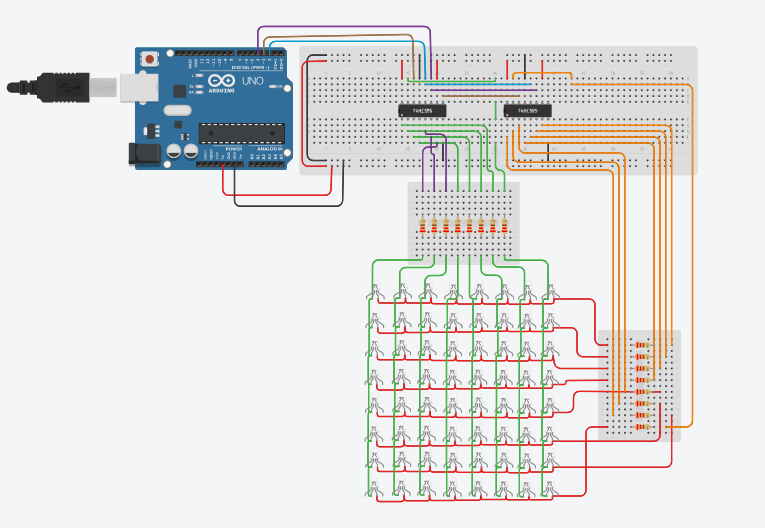
\includegraphics[width=8cm]{Imagen1.png}
    \centering
    \caption{Primer circuito}
    \label{fig:Imagen1}
\end{figure}\\\\

\textbf{\large Problema 2.}\\\\
Conectando los componentes de la forma planteada en la solucion del problema 1 se detectó que, al prender todos los leds (de forma "manual") se quemaban los circuitos integrados, no permitían un óptimo desarrollo del programa y se presentaban inconvenientes a la hora de realizar algunos patrones básicos (20/04/21).\\


\textbf{\large Solución}\\\\
Se rediseñó el circuito de tal manera que al seguir las compuertas lógicas de la siguiente tabla de verdad, los circuitos integrados no se quemaban, además de permitir (siguiendo la misma tabla de verdad) un diseño de algoritmo más eficiente y con posibilidad de ingresar cualquier patrón sin problema.\\

\begin{figure}[h]
    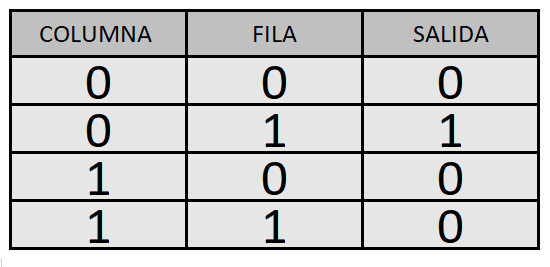
\includegraphics[width=8cm]{Tabla de verdad.png}
    \centering
    \caption{Tabla de verdad}
    \label{fig:Tabla de verdad}
\end{figure}\\\\

\begin{figure}[h]
    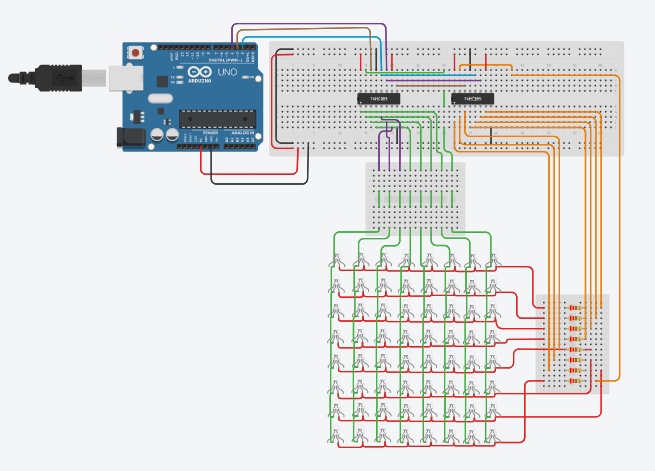
\includegraphics[width=8cm]{Imagen2.png}
    \centering
    \caption{Segundo circuito}
    \label{fig:Imagen2}
\end{figure}\\\\

\\
\\
\\
\textbf{\large Problema 3.}\\\\
Como recibir los patrones que el usuario quiera ingresar y traducir cada parte del patrón a la posición del led correspondiente (19/04/21).\\
\\\\\
\\

\textbf{\large Análisis}\\\\
Como idea principal se plantea nombrar e identificar cada posición de la matriz de leds, de forma que mediante una grafica mostrada en el manual de uso, el usuario pueda identificar que leds desea prender mediante el numero propio de cada led, además con el orden establecido de los números se puede dar la opción al usuario de prender varios leds al tiempo mediante un rango ingresado entre el 1 y el 64.
\\
\\
Ejemplo:
\\
\\
1\  \ 2\ \ \ 3\  \ 4\ \ \ 5\  \ 6\ \ \ 7\  \ 8\\ 
- \  \  - \  \ - \  \ - \  \ - \  \ - \  \ - \   \ -\\
- \  \  - \  \ - \  \ - \  \ - \  \ - \  \ - \   \ -\\
- \  \  - \  \ - \  \ - \  \ - \  \ - \  \ - \   \ -\\
- \  \  - \  \ - \  \ - \  \ - \  \ - \  \ - \   \ -\\
- \  \  - \  \ - \  \ - \  \ - \  \ - \  \ - \   \ -\\
- \  \  - \  \ - \  \ - \  \ - \  \ - \  \ - \   \ -\\
57 58 59 60 61 62 63 64\\

\textbf{\large Implementación}\\\\
\begin{figure}[h]
    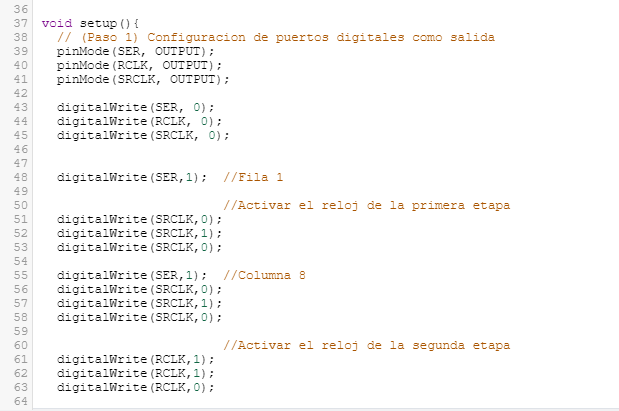
\includegraphics[width=8cm]{Imagen3.png}
    \centering
    \caption{Primer codigo (Recortado)}
    \label{fig:Imagen3}
\end{figure}\\\\

Después de inicializar las variables con el número del pin de salida, de configurar los puertos en modo OUTPUT y dejar las salidas en 0, se realizó el ingreso de cada dato con las posiciones de los leds correspondientes de forma manual, para poder experimentar con el funcionamiento e ir interiorizándolo, permitiendo crear patrones básicos.

\textbf{\large Problema 4.}\\\\



\end{document}